%!TEX program = xelatex
\documentclass[14pt]{article}
\usepackage{ctex}
\usepackage[utf8]{inputenc}
\usepackage{geometry}
\usepackage{amsmath,amssymb}
\usepackage{graphicx}
\usepackage{tikz}
\usepackage{wrapfig}
\usepackage{enumitem}
\geometry{a4paper, margin=2cm}

\setlist[enumerate]{label=\arabic*., left=0pt}

\begin{document}

\title{小学五年级奥林匹克数学竞赛试卷}
\author{}
\date{}
\maketitle

\section*{一、选择题}
\begin{enumerate}
\item 下列哪个数是质数?\\
\begin{tabular}{llll}
A. 21 & B. 33 & C. 47 & D. 57
\end{tabular}

\item 用一根36厘米长的铁丝围成一个正方形,边长是多少厘米?\\
\begin{tabular}{llll}
A. 6 & B. 7 & C. 8 & D. 9
\end{tabular}

\begin{wrapfigure}{r}{0.3\textwidth}
\centering
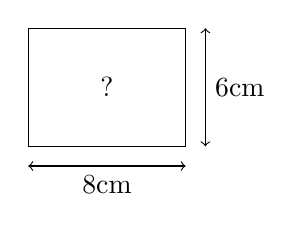
\begin{tikzpicture}[scale=0.5]
\draw (0,0)--(4,0)--(4,3)--(0,3)--cycle;
\node at (2,1.5) {?};
\draw[<->] (0,-0.5)--(4,-0.5) node[midway,below] {8cm};
\draw[<->] (4.5,0)--(4.5,3) node[midway,right] {6cm};
\end{tikzpicture}
\end{wrapfigure}

\item 右图长方形的面积是多少平方厘米?\\
\begin{tabular}{llll}
A. 24 & B. 36 & C. 48 & D. 54
\end{tabular}

\item 甲数是乙数的3倍,它们的和是120,乙数是多少?\\
\begin{tabular}{llll}
A. 20 & B. 30 & C. 40 & D. 60
\end{tabular}
\end{enumerate}

\section*{二、解答题}
\begin{enumerate}
\addtocounter{enumi}{4}

\item 鸡兔同笼,共有头12个,脚34只。问鸡兔各有多少只?
\vspace{6cm}

\item 右图三角形的面积是多少平方厘米?(要求写出计算过程)

\begin{wrapfigure}{r}{0.3\textwidth}
\centering
\begin{tikzpicture}[scale=0.4]
\draw (0,0)--(0,4)--(3,4)--cycle;
\node at (1.5,2) {面积?};
\draw[<->] (-0.5,0)--(-0.5,4) node[midway,left] {8cm};
\draw[<->] (0,-0.5)--(3,-0.5) node[midway,below] {6cm};
\end{tikzpicture}
\end{wrapfigure}
\vspace{6cm}

\item 现有1元硬币和5角硬币共30枚,总金额24元。求两种硬币各有多少枚?
\vspace{6cm}
\end{enumerate}

\newpage
\section*{参考答案}

\subsection*{选择题}
\begin{enumerate}
\item C \quad 47是质数
\item D \quad $36\div4=9$
\item C \quad $8\times6=48$
\item B \quad 设乙数为x,则$3x+x=120$,解得$x=30$
\end{enumerate}

\subsection*{解答题}
\begin{enumerate}
\setcounter{enumi}{4}
\item 鸡7只,兔5只\\
(解:设鸡x只,兔y只\\
$\begin{cases}
x+y=12 \\
2x+4y=34
\end{cases}$\\
解得$x=7$, $y=5$)

\item 面积24平方厘米\\
(解:$8\times6\div2=24$)

\item 1元硬币18枚,5角硬币12枚\\
(解:设1元x枚,则5角(30-x)枚\\
$1x + 0.5(30-x) = 24$\\
解得$x=18$)
\end{enumerate}

\end{document}